%%%%%%%%%%%%%%%%%%%%%%%%%%%%%%%%%%%%%%%%%%%%%%%%%%%%%%%%%%%%%%%%%%%%%%%
%%%%  Load the document class and packages                         %%%%
%%%%%%%%%%%%%%%%%%%%%%%%%%%%%%%%%%%%%%%%%%%%%%%%%%%%%%%%%%%%%%%%%%%%%%%
\documentclass[a4paper]{report}
\usepackage{epsfig}            % to insert PostScript figures
\graphicspath{ 
  {figures/} 
}

%Change figure names
\renewcommand{\figurename}{Fig}

\usepackage[bf,footnotesize]{caption} % make captions small and label bold


\addtocounter{chapter}{1} %Because starting at zero is silly
\makeatletter
\renewcommand{\thesection}{\@arabic\c@section}
\renewcommand{\thefigure}{\@arabic\c@figure}
\makeatother

\usepackage[a4paper,margin=2.7cm,tmargin=2.5cm,bmargin=2.5cm]{geometry} 
\usepackage{textcomp}          % To make nice degree symbols and others\usepackage[bf,footnotesize]{caption} % make captions small and label bold
\usepackage{wrapfig}
%to produce the clickable references along the left in Acroread. This
%package must be included last. 
\usepackage[ps2pdf,bookmarks=TRUE]{hyperref} 



%%%%%%%%%%%%%%%%%%%%%%%%%%%%%%%%%%%%%%%%%%%%%%%%%%%%%%%%%%%%%%%%%%%%%%%
%%%%  Hypertext references for Acrobat                             %%%%
%%%%%%%%%%%%%%%%%%%%%%%%%%%%%%%%%%%%%%%%%%%%%%%%%%%%%%%%%%%%%%%%%%%%%%%
\hypersetup{
pdfauthor = {TENSS},
pdftitle = {Laser Alignment},
pdfkeywords = {lasers,optics,alignment,reflection,microscopy},
pdfcreator = {LaTeX with hyperref},
pdfproducer = {dvips + ps2pdf}
           }


\begin{document}




%set the number of sectioning levels 
\setcounter{secnumdepth}{2}

\begin{center}
\textbf{\Large{Laser Routing and Alignment}}
\end{center}

In most situations the laser is in a fixed position but its beam must pass precisely through a series of optical elements. 
We use small flat \textit{first surface} mirrors to route the beam through the required path. 
Fine position of the beam, e.g. along an optical axis defined by a beam expander, is a critical skill for building a microscope. 
The aim of this exercise is to use mirrors to redirect a laser beam coming in at an arbitrary angle through a specific line at a specific height above the table.
Do not touch the mirror surfaces! 
They are delicate.


\section{Exercise 1}

\begin{figure}[h]
\center
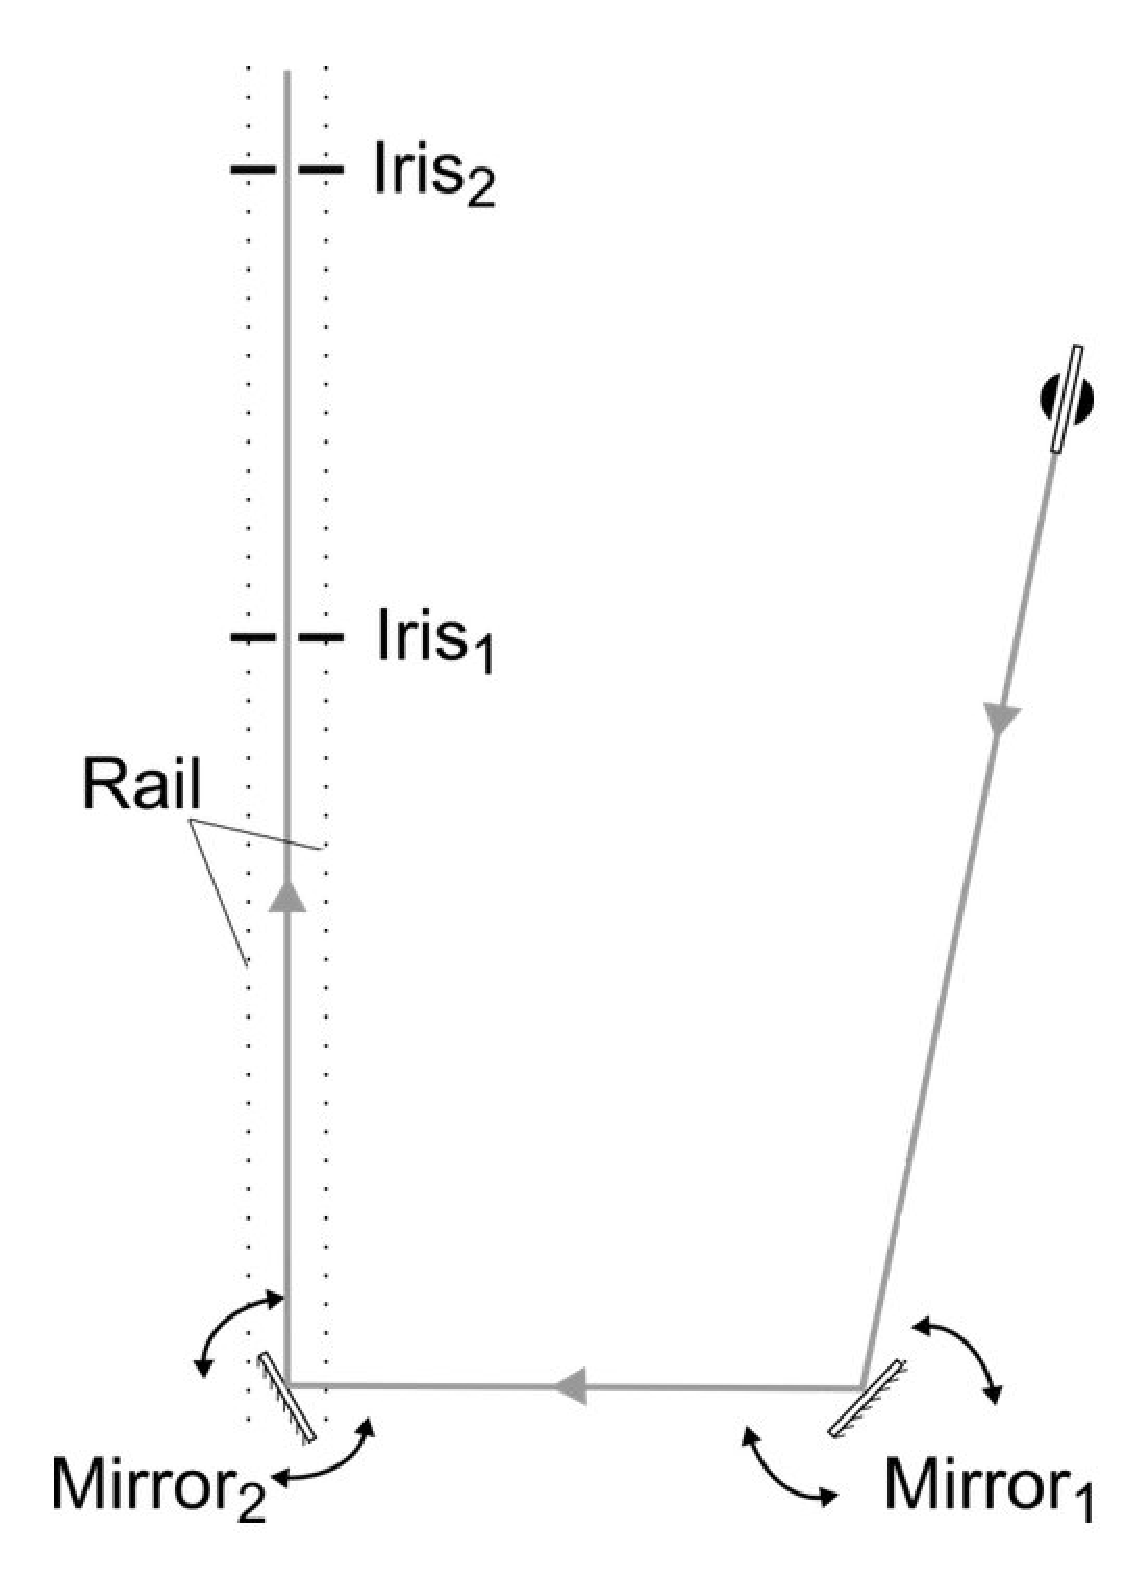
\includegraphics[width=4in]{laser_alignment_exercise_basic.eps}
\caption{}
\label{fig:ex1}
\end{figure}

Set the components as shown in Fig.~\ref{fig:ex1}. 
The goal is to align the laser to pass through the two iris centres without moving or adjusting the laser pointer. 
To complete the exercise you will need to understand the following keys points:

\begin{enumerate}
\item Adjusting mirror 1 translates the beam across the surface of mirror 2.
\item Adjusting mirror 2 alters the angle with which the beam goes through the irises. 
\item As a consequence of (1), you adjust mirror 1 to pass the beam through iris 1.
\item As a consequence of (2), you adjust mirror 2 to pass the beam through iris 2.
\item Iterating steps (3) and (4) will allow the beam to pass through both irises, assuming that there exists a region of mirror 2 that falls along the axis defined by the two irises. 
\end{enumerate}


Here is how you will implement the above:

\begin{enumerate}
\item Close iris 1 and rotate mirror 1 to position beam at the centre of iris 1.
\item Open iris 1 and rotate mirror 2 to position beam at centre of closed iris 2. 
The process of doing this will move the beam away from the centre of iris 1. 
The degree to which this happens depends on the distance between mirror 2 and iris 1.
\item Close iris 1 and assess the beam position. If not aligned, repeat steps 1 \& 2. 
If aligned, stop. 
\end{enumerate}

\subsubsection{Notes}

The above procedure is guaranteed to converge on a correctly aligned path if such a path is physically possible. 
\texfbf{Tip:} If after repeated attempts at alignment you keep failing, this indicates that a mirror (probably mirror 2) is mis-positioned. 

In general, two mirrors are all you need to align a beam to a desired line in space. 
To make your task easier, you need two landmarks that define the desired alignment line. 
In the case above, these were the two irises. 
But potentially you can use any two reference points that lie on your axis of interest. 
Note that these landmarks must be situated after both the mirrors.

The general rule is always:
\begin{itemize}
\item Tweak the first mirror (mirror closer to the laser source, mirror 1) to align the beam on the first
landmark (landmark closer to the laser, landmark 1).
\item Tweak the second mirror (mirror farther from the laser source, mirror 2) to align the beam on
the second landmark (landmark 2).
\end{enumerate}

Useful rules of thumb:
\begin{itemize}
\item Only use right angles. 
Whilst it is possible to use very acute angles and still solve the alignment task, you will have a larger mirror area to play with if you reflect the beam at 90 degree angles.
\item Manage your real-estate: You will notice that sometimes, the beam will fall off mirror 2. This problem can be solved by using a larger mirror, or by translating mirror 2 in the direction where the beam fell off its edge. It usually helps to keep all reflection angles close to 90 degrees to minimise running out of mirror space!
\end{itemize}


\section{Exercise 2}
Your 2-photon laser has arrived and it's time to begin building your microscope's light path. 
To make your life easier, you decide to use two mirrors to ensure that the beam emerging from the laser comes out parallel with the optical table and at a height suitable for your lenses and other optical elements. 
Set up your laser pointer and two mirrors as shown in Fig.~\ref{fig:ex2}. 
The mirrors can be as close to the laser as you like. 
Place and iris on a post holder and use a post base to improve stability. 
Do not bolt the iris to the table.
This single iris defines the height at which you want the beam to be at all locations on the optical table. 
Based on what you learned in Exercise 1, use the iris and the two mirrors to the beam is parallel with the table at the height defined by your iris. 
Hint: all you're allowed to do is change the tilt of the two mirrors and move the position of the iris (which is not bolted to the table).


\begin{figure}[h]
\center
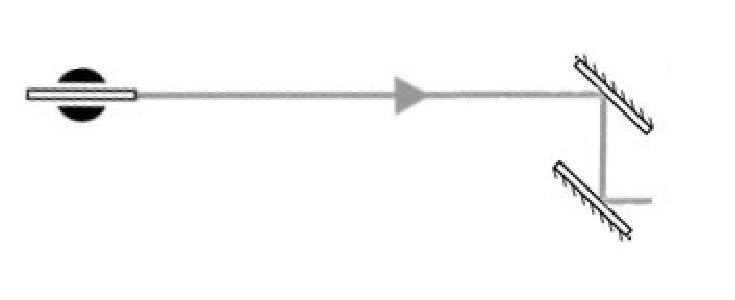
\includegraphics[width=4in]{laser_height.eps}
\caption{}
\label{fig:ex2}
\end{figure}



\end{document}
